
\def \Subject {پروژه}
\def \Course {درس معماری کامپیوتر}
\def \Report {طراحی پردازنده FUM-MIPS}
% \def \StudentNumber {98524044}

\begin{center}
\vspace{.4cm}
{\bf {\huge \Subject}}\\
{\bf \Large \Course}
\vspace{.2cm}
\end{center}
% {\bf \Author }  \\
% \hspace{} 
{\bf مهلت تحویل تا: \date{1402/04/01}}    
\hspace{\fill} 
{\bf \Report} \\
\hrule
\vspace{0.8cm}

%\huge{\Subject}\\[1.5 cm]
%\chapterauthor{\Author~ : \StudentNumber}
\begin{itemize}
    \item پروژه به صورت گروهی است. (گروه های دو نفره) 
    \item در سامانه ویو فایل‌های ویدئویی و متنی برای یادآوری و آموزش کار با verilog قرار گرفته است.
    \item  محتویات پروژه را به صورت یک فایل با فرمت : \\\lr{\small{FirstnameLastname\_StudentNumber\_FirstnameLastname\_StudentNumber.zip}}\\ بارگذاری کنید.
    \\(مثال (MohammadMohammadi\_9XXXXXX\_RezaRezaei\_9XXXXXX.zip
    \item کامنت گذاری تمام خطوط کد الزامی است.
    \item تحویل پروژه بعد از مهلت مشخص شده نمره ای نخواهد داشت.
    \item در صورت اثبات کپی برداری، نمره پروژه کپی شده و کپی شونده هر دو از ۱۰۰ نمره، ۱۰۰- خواهد بود.
    \item زمانبندی تحویل آنلاین پروژه پس از اتمام مهلت ارسال اعلام خواهد شد.
    \item تحویل پروژه از طریق تلگرام، ایمیل و ... امکان پذیر نیست.
\end{itemize}

\section*{هدف}
{در این آزمایش، به طراحی و مدل‌سازی یک پردازنده تک سیکل با زبان verilog می پردازیم. نام این پردازنده FUM-MIPS می باشد.}\\
{FUM-MIPS یک پردازنده ۱۶ بیتی بوده که در این پردازنده بانک ثبات شامل ۸ ثبات ۱۶ بیتی می باشد. معماری مجموعه دستورات (ISA)\footnote{\lr{Instruction Set Architecture}} این پردازنده شبیه به ISA پردازنده MIPS می باشد ولی تفاوت هایی نسبت به آن دارد. طول دستورات در این پردازنده ۱۶ بیت می‌باشد. یعنی شمارنده برنامه (PC)\footnote{\lr{Program Counter}} به جای اینکه با ۴ جمع شود باید با ۲ جمع شود. PC یک ثبات ۱۶ بیتی می‌باشد. در این پردازنده سه نوع ماشین کد وجود دارد که عبارتنداز: \lr{R-Type}، \lr{I-Type} و \lr{J-Type} .}\\
\begin{center}
    \chapter\LARGE{معرفی FUM-MIPS}\\
\end{center}\\
\section{دستورات R-Type}
{دستورات R-Type مانند دستورات R-Type در MIPS می‌باشد. دو source و یک مقصد دارند. ماشین کد دستورات R-Type به شکل زیر می‌باشد.}\\
{چهار بیت اول (بیت‌های ۱۲ الی ۱۵) opcode را مشخص می‌کند که opcode برای دستورات R-Type صفر ("0000") می‌باشد.}\\
{سه بیت بعد (بیت‌های ۹ الی ۱۱) شماره ثبات برای مبدأ اول را مشخص می‌کند. سه بیت بعد (بیت‌های ۶ الی ۸) شماره ثبات برای مبدأ دوم را مشخص می‌کند. سه بیت بعد (بیت‌های ۳
الی ۵)  شماره ثبات مقصد را مشخص می‌کند و سه بیت آخر (بیت‌های صفر الی ۲) نوع عملیات را مشخص می‌کند.}\\
{مقادیر
function برای دستورات \lr{add}، \lr{sub}، \lr{and}، \lr{or}، \lr{xor}، \lr{nor} و slt در جدول ۲ آمده است.
}
\begin{table}[H]
    \centering
    \begin{tabular}{|c|c|c|c|c|}
    \hline
    ۲−۰ & ۵−۳ & ۸−۶ & ۱۱−۹ & ۱۵−۱۲ \\
    \hline
    ۳−bit & ۳−bit & ۳−bit & ۳−bit & ۴−bit \\
    \hline
    function & destination & source۲ & source۱ & opcode \\
    \hline
    \end{tabular}
    \caption{قالب دستورات R-Type}
    \label{R-Type-Instructions-Template}
\end{table}

\begin{table}[H]
    \centering
    \begin{tabular}{|c|c|}
    \hline
    function & operation \\
    \hline
    000 & add \\
    \hline
    001 & sub \\
    \hline
    010 & and \\
    \hline
    011 & or \\
    \hline
    100 & xor \\
    \hline
    101 & nor \\
    \hline
    110 & slt \\
    \hline
    \end{tabular}
    \caption{مقادیر opcode و function برای دستورات R-Type}
    \label{R-Type-Opcode-Values}
\end{table}
\begin{LTR}
    \noindent{assembly:}\\
    \indent{add reg1\lr{,} reg2\lr{,} reg3}\\
    {semantics:}\\
    \indent{GPR[reg1] --> GPR[reg2] + GPR [reg3]}\\
    \indent{PC --> PC + 2}
\end{LTR}
\section{دستورات I-Type}
{دستورات I-Type مانند دستورات I-Type در MIPS می‌باشد با این تفاوت که مقدار immediate شش بیتی می‌باشد. کد ماشین دستورات I-Type در جدول ۳ آورده شده است.}\\
{چهار بیت اول (بیت‌های ۱۲ الی ۱۵) opcode را مشخص می‌کند. سه بیت بعد (بیت‌های ۹ الی ۱۱) شماره ثبات را مشخص می‌کند. سه بیت بعد (بیت‌های ۶ الی ۸) شماره ثبات دوم را مشخص می‌کند. شش بیت آخر (بیت‌های صفر الی ۵) مقدار immediate را مشخص می‌کند.}\\
{برای دستورات \lr{addi}، \lr{subi}، ori و andi چهار بیت اول (بیت‌های ۱۲ الی ۱۵) opcode را مشخص می‌کند. سه بیت بعد (بیت‌های ۹ الی ۱۱) شماره ثبات مبدأ را مشخص می‌کند. سه بیت بعد (بیت‌های ۶ الی ۸) شماره ثبات مقصد را مشخص می‌کند. شش بیت آخر (بیت‌های صفر الی ۵) مقدار immediate را مشخص می‌کند. این مقدار ۶ بیتی برای دستورات addi و subi توسعه علامت (\lr{sign extend}) می‌شود و برای دستورات ori و andi عمل توسعه با صفر (\lr{zero extend}) صورت می‌گیرد و به یک مقدار ۱۶ بیتی تبدیل شده و بعد با محتوای ثبات عملیات انجام می‌شود. مقادیر opcode برای دستورات \lr{addi}، \lr{subi}، andi و ori در جدول ۴ آمده است.}\\
\begin{table}[H]
    \centering
    \begin{tabular}{|c|c|c|c|}
    \hline
    ۵−۰ & ۸−۶ & ۱۱−۹ & ۱۵−۱۲ \\
    \hline
    ۶−bit & ۳−bit & ۳−bit & ۴−bit \\
    \hline
    Immediate & register۲ & register۱ & opcode \\
    \hline
    \end{tabular}
    \caption{قالب دستورات I-Type}
    \label{I-Type-Instructions-Template}
\end{table}

\begin{table}[H]
    \centering
    \begin{tabular}{|c|c|}
    \hline
    opcode & operation \\
    \hline
    0001 & addi \\
    \hline
    0010 & andi \\
    \hline
    0011 & ori \\
    \hline
    0100 & subi \\
    \hline
    \end{tabular}
    \caption{مقادیر opcode برای دستورات \lr{addi}، \lr{subi}، \lr{andi} و ori}
    \label{I-Type-Opcode-Values}
\end{table}
\begin{LTR}
    \noindent{assembly:}\\
    \indent{addi Reg1\lr{,} Reg2\lr{,} Imm}\\
    {semantics:}\\
    \indent{GPR[Reg1] --> GPR[Reg2] + {sign-extend(Imm)}}\\
    \indent{PC --> PC + 2}\\
\\
    \noindent{assembly:}\\
    \indent{andi Reg1\lr{,} Reg2\lr{,} Imm}\\
    {semantics:}\\
    \indent{GPR[Reg1] --> GPR[Reg2] + {zero-extend(Imm)}}\\
    \indent{PC --> PC + 2}\\
\end{LTR}

\noindent{برای این پردازنده دستورات \lr{load (lhw)} و \lr{store (shw)} جزء قالب I-Type حساب می‌شوند. دستورات lhw , shw به ترتیب یک داده ۱۶ بیتی را از حافظه می‌خواند و یک داده ۱۶ بیتی را در حافظه می‌نویسد.}\\
{در این پردازنده مانند MIPS از آدرس دهی displacement (محتوای ثبات + \lr{offset}) برای محاسبه آدرس استفاده می‌شود.}\\
{برای دستورات lhw چهار بیت اول (بیت‌های ۱۲ الی ۱۵) opcode را مشخص می‌کند. سه بیت بعد (بیت‌های ۹ الی ۱۱) شماره ثبات پایه را مشخص می‌کند. سه بیت بعد (بیت‌های ۶ الی ۸) شماره ثبات مقصد را مشخص می‌کند. شش بیت آخر (بیت‌های صفر الی ۵) مقدار offset را مشخص می‌کند که باید \lr{sign extend} شود و بعد با ثبات پایه جمع شود و آدرس را تولید کند.}\\
{برای دستورات shw چهار بیت اول (بیت‌های ۱۲ الی ۱۵) opcode را مشخص می‌کند. سه بیت بعد (بیت‌های ۹ الی ۱۱) شماره ثبات پایه را مشخص می‌کند. سه بیت بعد (بیت‌های ۶ الی ۸) شماره ثبات مبدأ را مشخص می‌کند. شش بیت آخر (بیت‌های صفر الی ۵) مقدار offset را مشخص می‌کند که باید \lr{sign extend} شود و بعد با ثبات پایه جمع شود و آدرس را تولید کند. مقدار offset یک مقدار علامت‌دار\footnote{signed} می‌باشد. مقادیر opcode برای دستورات lhw و shw ، در جدول ۵ آمده است.}\\
\begin{table}[H]
    \centering
    \begin{tabular}{|c|c|}
    \hline
    opcode & operation \\
    \hline
    0111 & lhw \\
    \hline
    1000 & shw \\
    \hline
    \end{tabular}
    \caption{مقادیر opcode برای دستورات lhw و shw}
    \label{lhw-shw-Opcode-Values}
\end{table}
\begin{LTR}
    \noindent{assembly:}\\
    \indent{lhw reg1\lr{,} Imm(Reg2)}\\
    {semantics:}\\
    \indent{EA --> GPR[Reg2] + sign-extend(imm)}\\
    \indent{GPR[Reg1] --> Memory[EA]}\\ 
    \indent{PC --> PC + 2}\\
\\
    \noindent{assembly:}\\
    \indent{shw reg1\lr{,} Imm(Reg2)}\\
    {semantics:}\\
    \indent{EA --> GPR[Reg2] + sign-extend(imm)}\\
    \indent{Memory[EA] --> GPR[Reg1]}\\
    \indent{PC --> PC + 2}\\
\end{LTR}
{برای این پردازنده دستورات پرش (‌Branch) جز قالب I-Type حساب می‌شوند. دستورات پرش محتوای دو ثبات را با یکدیگر مقایسه می‌کنند و براساس نوع مقایسه، اگر نتیجه درست باشد پرش انجام می‌شود و در غیر اینصورت انجام نمی‌شود. آدرس پرش به اینصورت محاسبه می‌شود که مقدار شش بیتی immediate به مقدار ۱۶ بیتی \lr{sign extend} می‌شود سپس در دو ضرب می‌گردد و بعد با PC+2 جمع می‌شود. نتیجه این جمع آدرس محل پرش را مشخص می‌کند:}
$$ (PC+2+(sign extend (imm)\times 2)) $$
{جدول ۶ انواع دستورات پرش و opcode آنها را نشان می‌دهد.}\\
\begin{table}[H]
    \centering
    \begin{tabular}{|c|c|c|}
    \hline
    operation & instruction & opcode \\
    \hline
    \lr{Branch if equal} & beq & 1001 \\
    \hline
    \lr{Branch if not equal} & bne & 1010 \\
    \hline
    \lr{Branch if less than} & blt & 1011 \\
    \hline
    \lr{Branch if greater than} & bgt & 1100 \\
    \hline
    \end{tabular}
    \caption{مقادیر opcode برای دستورات پرش}
    \label{Jump-Instructions-Opcode}
\end{table}
\begin{LTR}
    \noindent{assembly:}\\
    \indent{beq reg1\lr{,} reg2\lr{,} imm}\\
    {semantics:}\\
    \indent{if GPR[reg1] == GPR[reg2] then}\\
    \indent\indent{PC --> PC + 2 + (sign-extend(imm)*2)}\\
    \indent{else}\\
    \indent\indent{PC --> PC + 2}\\
\end{LTR}
\section{دستورات J-Type}
{دستور jmp از نوع J-Type می‌باشد. ماشین کد دستورات J-Type در جدول ۷ آورده شده است. در این دستور ۱۲ بیت پایین دستور (بیت‌های صفر الی ۱۱) در ۲ ضرب می‌شود (تبدیل به یک مقدار ۱۳ بیتی می‌شود) و سپس سه بیت بالای PC به ابتدای آن اضافه می‌شود تا یک مقدار ۱۶ بیتی ایجاد گردد و سپس در PC نوشته می‌شود. opcode دستور jmp برابر "1111" می‌باشد.}\\
\begin{LTR}
    \noindent{assembly:}\\
    \indent{jmp label}\\
    {semantics:}\\
    \indent{PC --> PC[15:13] \&\& (instr[11:0]) \&\& "0"}\\
\end{LTR}
\begin{table}[H]
    \centering
    \begin{tabular}{|c|c|}
    \hline
    ۱۱−۰ & ۱۵−۱۲ \\
    \hline
    12-bit & 4-bit \\
    \hline
    \lr{jump address} & \lr{Opcode (1111)} \\
    \hline
    \end{tabular}
    \caption{قالب دستورات J-Type}
    \label{J-Type-Instructions-Template}
\end{table}
\section{ماژول ها}
\subsection{\lr{Register file}}
{شکل ۱ بلوک دیاگرام این ماژول را نشان می‌دهد. ورودی های \lr{read register 1}، \lr{read register 2} و \lr{write register} سه بیتی می‌باشند که آدرس‌های ثبات‌های خوانده شده و نوشته شده را مشخص می‌کنند. ورودی regwrite هم به عنوان سیگنال فعالساز (enable) برای بانک ثبات عمل می‌کند. این بانک ثبات یک ورودی کلاک هم دارد که با لبه بالارونده عمل می‌کند. هرگاه سیگنال regwrite در لبه بالارونده کلاک یک باشد عمل نوشتن در ثبات انجام می‌شود. ورودی \lr{write data} باید یک ورودی ۱۶ بیتی باشد که داده‌ای را که باید در ثبات نوشته شود مشخص می‌کند. خروجی‌های \lr{read data 1} و \lr{read data 2} خروجی‌های ۱۶ بیتی هستند که مقادیر ثبات‌های \lr{read register 1} و \lr{read register 2} را شامل می‌شوند.}\\
\begin{figure}[H]
    \centering
    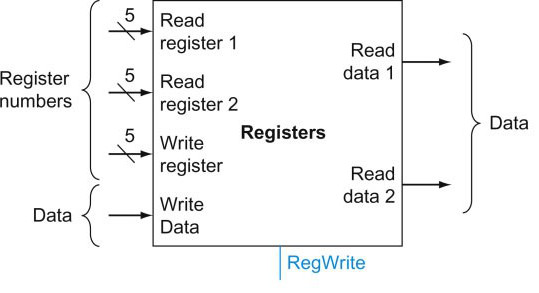
\includegraphics[width=\textwidth]{images/MIPS_Register_File.jpg}
    \caption{بانک ثبات}
    \label{Register_Bank}
\end{figure}\\

\subsection{ALU}
{شکل ۲ بلوک دیاگرام این ماژول را نشان می‌دهد. دو ورودی ALU باید ۱۶ بیتی و خروجی \lr{ALU result} نیز باید ۱۶ بیتی باشند. ورودی چهاربیتی \lr{ALU opration} مشخص می‌کند که ALU چه عملی انجام دهد. خروجی یک بیتی zero اگر یک باشد نشان می‌دهد که مقدار \lr{ALU result} صفر می‌باشد. ALU شما بجز خروجی zero باید شامل دو خروجی تک بیتی \lr{lt (less than)} و \lr{gt (greater than)} نیز باشد. اگر data1 از data2 بزرگتر باشد خروجی gt باید یک شود و اگر data1 از data2 کوچکتر باشد خروجی lt باید یک شود.}\\
\begin{figure}[H]
    \centering
    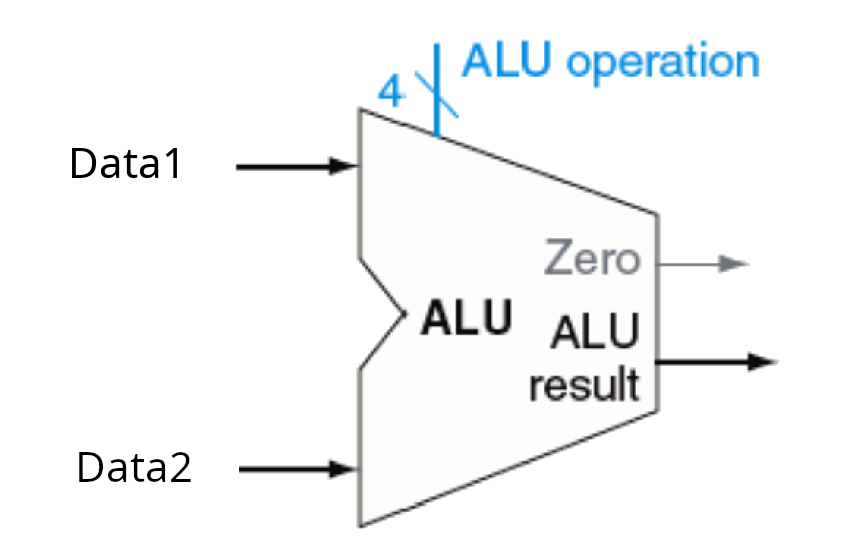
\includegraphics[width=0.7\textwidth]{images/MIPS_ALU.png}
    \caption{ALU}
    \label{MIPS_ALU}
\end{figure}\\

\subsection{حافظه داده}
{شکل ۳ بلوک دیاگرام این ماژول را نشان می‌دهد. ورودی address و \lr{write data} و خروجی \lr{read data} مقادیر ۱۶ بیتی می‌باشند. دو سیگنال ورودی کنترل MemRead و MemWrite یک بیتی می‌باشند که اگر یک باشند به ترتیب عمل خواندن از حافظه و نوشتن در حافظه انجام می‌شود.}
\begin{figure}[H]
    \centering
    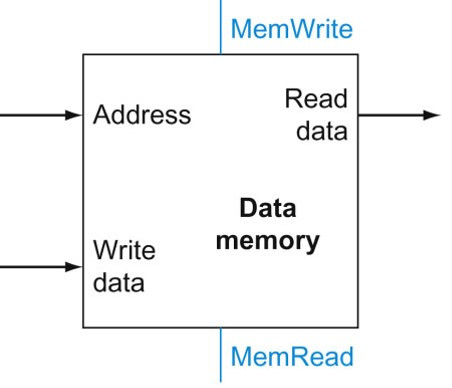
\includegraphics[width=0.6\textwidth]{images/Data_Memory.jpg}
    \caption{حافظه داده}
    \label{Data_Memory}
\end{figure}\\
\subsection{حافظه برنامه}
{شکل ۴ بلوک دیاگرام این ماژول را نشان می‌دهد. ورودی address و خروجی instruction مقادیر ۱۶ بیتی می‌باشند. برای این پروژه فرض کنید که حافظه حداکثر ۲۵۶ خانه ۱۶ بیتی دارد.}
\begin{figure}[H]
    \centering
    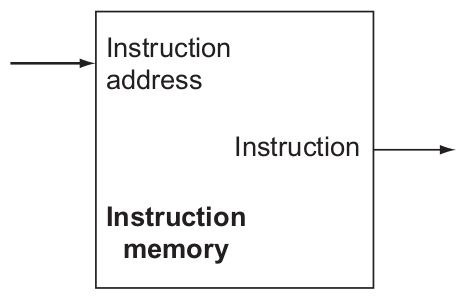
\includegraphics[width=0.6\textwidth]{images/MIPS_Instruction_Memory.png}
    \caption{حافظه برنامه}
    \label{Instruction_Memory}
\end{figure}\\
\section{پیاده‌سازی}
{\Large\textcolor{red}{دقت داشته باشید که این دو فاز به صورت مجزا در ویو تحویل داده می شوند. بنابراین هر فاز باید به طور مجزا قابل اجرا باشد.}\\}
\subsection{فاز اول: پردازنده تک‌سیکل \lr{(Single Cycle)}}
{در فاز اول دانشجویان باید پردازنده تک‌سیکل را در دو مرحله پیاده‌سازی کنند.}
\subsubsection{مرحله اول}
{در مرحله اول انجام آزمایش دانشجویان باید با استفاده از ماژول‌های ذکر شده و اضافه کردن واحد کنترل، PC و ماژول‌های مورد نیاز، طراحی کلی پردازنده را نهایی کنند (پردازنده‌ای مشابه شکل ۵) تا بتوانند دستورات ذکر شده را اجرا کنند.}\\
{دانشجویان باید در یک محیط شبیه‌سازی نشان دهند که پردازنده طراحی شده به درستی تمام دستورات را اجرا می‌کند.}\\
\subsubsection{مرحله دوم}
{در این مرحله دانشجویان باید برنامه ای بنویسند که بتواند در یک آرایه با ۹ عنصر که شامل داده‌های ۱۶ بیتی می‌باشد، بزرگترین و کوچکترین و میانه اعداد را بدست آورد. نمایش صحت درستی اجرای برنامه بر روی یک محیط شبیه سازی (مانند Modelsim و یا \lr{Verilator}) باید نمایش داده شود.}\\

\subsection{فاز دوم: پردازنده پایپلاین (Pipeline)}
{در این فاز باید پروژه فاز قبل را پایپلاین کنید. همچنین باید هازارد های داده را رفع کنید. رفع هازارد های کنترلی ممکن است به نمره اضافه منجر شود.}\\
{توجه:}\\
{برای انجام فاز دوم، بعد از انجام فاز اول و بارگذاری آن در ویو، فاز اول را کپی کرده و به عنوان یک پروژه جدید باز کنید و سپس تغییرات لازم برای تبدیل فاز اول به فاز دوم را اعمال کنید. }\\
\begin{figure}[H]
    \centering
    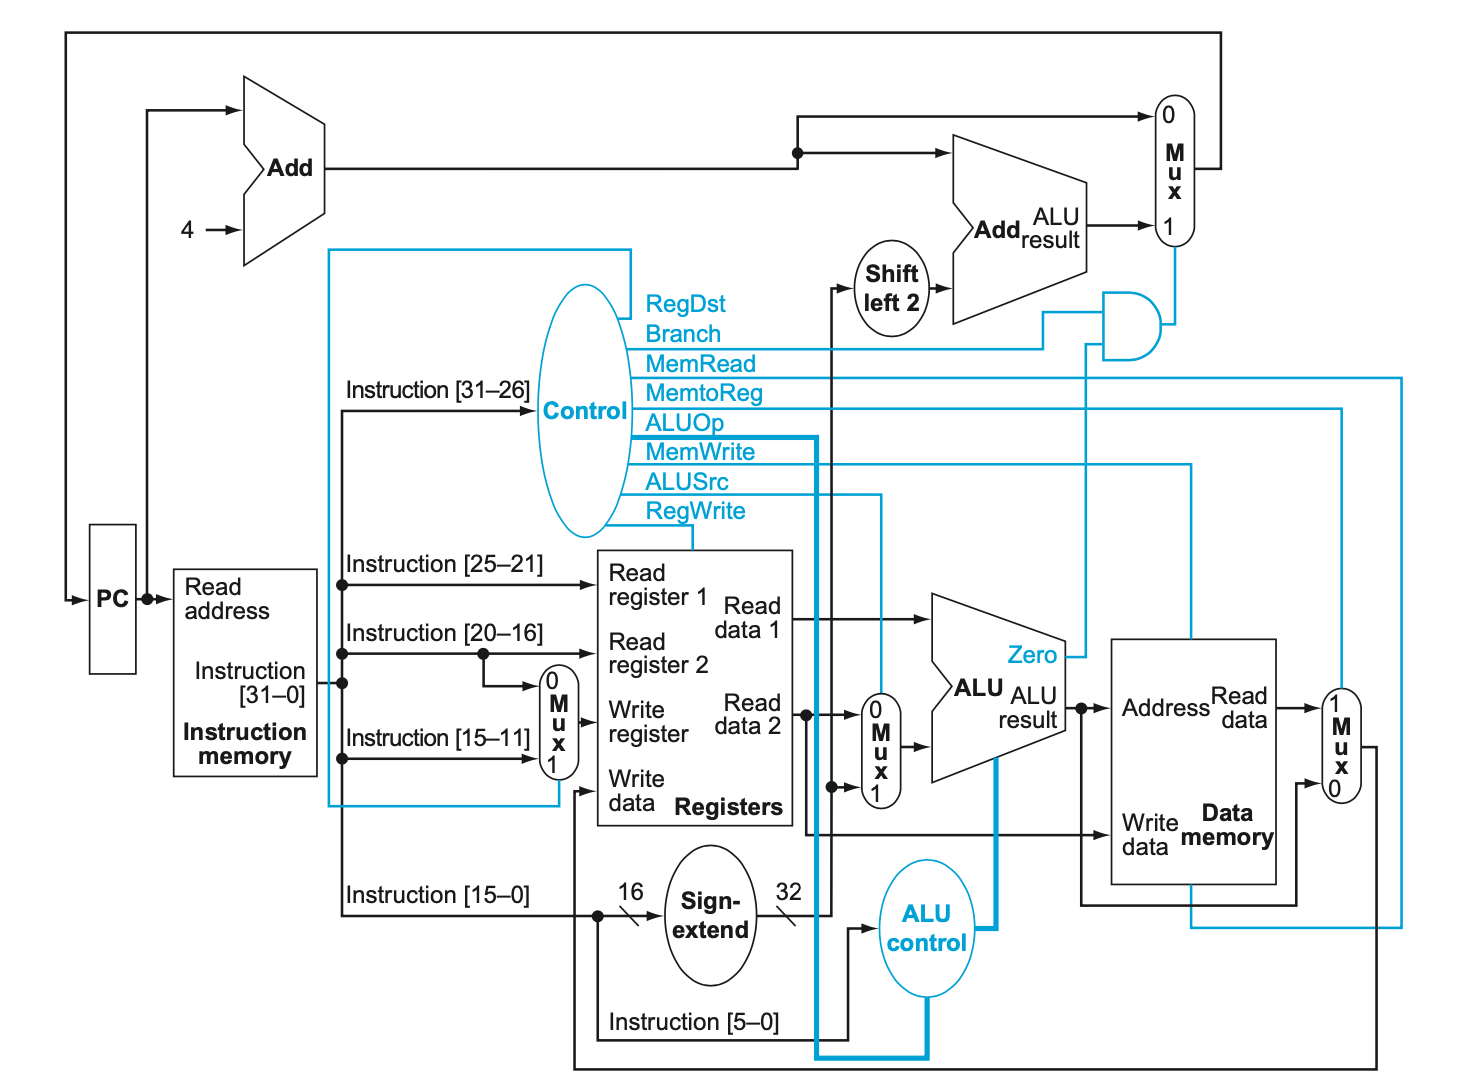
\includegraphics[width=\textwidth]{images/MIPS_Single_Cycle_Processor.png}
    \caption{نمای کلی پردازنده}
    \label{MIPS_Single_Cycle_Processor}
\end{figure}\\







